%
% File emnlp2018.tex
%
%% Based on the style files for EMNLP 2018, which were
%% Based on the style files for ACL 2018, which were
%% Based on the style files for ACL-2015, with some improvements
%%  taken from the NAACL-2016 style
%% Based on the style files for ACL-2014, which were, in turn,
%% based on ACL-2013, ACL-2012, ACL-2011, ACL-2010, ACL-IJCNLP-2009,
%% EACL-2009, IJCNLP-2008...
%% Based on the style files for EACL 2006 by 
%%e.agirre@ehu.es or Sergi.Balari@uab.es
%% and that of ACL 08 by Joakim Nivre and Noah Smith

\documentclass[11pt,a4paper]{article}
\usepackage[hyperref]{emnlp2018}
\usepackage{times}
\usepackage{latexsym}

\usepackage{url}
 \usepackage{multirow}
\usepackage{tikz}
\usetikzlibrary{calc, positioning, arrows, automata,fit,shapes.geometric,backgrounds,shapes.misc}
\usepackage{tikz-dependency}
\usepackage{pgfplots}
\pgfplotsset{compat=1.12}
\usepackage{amsthm}
\usepackage{framed}
\usepackage{caption}
\usepackage{subcaption}
\usepackage{graphicx}
\usepackage{xcolor,colortbl}
\usepackage{algorithm2e}
\usepackage{amsmath}
%\usepackage{authblk}

\aclfinalcopy % Uncomment this line for the final submission
%\def\aclpaperid{***} %  Enter the acl Paper ID here

%\setlength\titlebox{5cm}
% You can expand the titlebox if you need extra space
% to show all the authors. Please do not make the titlebox
% smaller than 5cm (the original size); we will check this
% in the camera-ready version and ask you to change it back.

\mathchardef\mhyphen="2D
\DeclareMathOperator*{\argmax}{arg\,max}


\newcommand{\squishlist}{
 \begin{list}{--}
  { \setlength{\itemsep}{0pt}
     \setlength{\parsep}{3pt}
     \setlength{\topsep}{3pt}
     \setlength{\partopsep}{0pt}
     \setlength{\leftmargin}{1.5em}
     \setlength{\labelwidth}{1em}
     \setlength{\labelsep}{0.5em} } }

\newcommand{\squishend}{
  \end{list}  }
 
 
\definecolor{Gray}{gray}{0.85}
\definecolor{lGray}{gray}{0.95}
\newcommand{\GG}[1]{}
  \newcolumntype{a}{>{\columncolor{lGray}}r}
\newcolumntype{b}{>{\columncolor{lGray}}r}

\newcommand\BibTeX{B{\sc ib}\TeX}
\newcommand\confname{EMNLP 2018}
\newcommand\conforg{SIGDAT}

\title{Using Linguistic Features to Improve the Generalization Capability \\of Neural Coreference Resolvers}

\author{Nafise Sadat Moosavi$^{1,2}$\thanks{\hspace{0.7em}This author is currently employed by the Ubiquitous Knowledge Processing (UKP) Lab, Technische Universit\"at Darmstadt,  https://www.ukp.tu-darmstadt.de.} \and Michael Strube$^{1}$
       \\
       $^1$Heidelberg Institute for Theoretical Studies gGmbH\\
       $^2$Research Training Group AIPHES\\
	   %\small \url{{nafise.moosavi|michael.strube}@h-its.org}\\
	   \small \url{moosavi@ukp.informatik.tu-darmstadt.de}, \url{michael.strube@h-its.org}}
	   

\date{}

\begin{document}
\maketitle
\begin{abstract}
Coreference resolution is an intermediate step for text understanding.
It is used in tasks and domains for which we do not necessarily have coreference annotated corpora.
Therefore, generalization is of special importance for coreference resolution.
However, while recent coreference resolvers have notable improvements on the CoNLL dataset,
they struggle to generalize properly to new domains or datasets.
In this paper, we investigate the role of linguistic features in building more generalizable coreference resolvers.
We show that generalization improves only slightly by merely using a set of additional linguistic features.
However, employing features and subsets of their values that are informative for coreference resolution,
considerably improves generalization.
Thanks to better generalization, our system
achieves state-of-the-art results in out-of-domain evaluations,
e.g., on WikiCoref, 
our system, which is trained on CoNLL, achieves on-par performance with a system designed for this dataset.

\end{abstract}

% !TEX root = ../arxiv.tex

Unsupervised domain adaptation (UDA) is a variant of semi-supervised learning \cite{blum1998combining}, where the available unlabelled data comes from a different distribution than the annotated dataset \cite{Ben-DavidBCP06}.
A case in point is to exploit synthetic data, where annotation is more accessible compared to the costly labelling of real-world images \cite{RichterVRK16,RosSMVL16}.
Along with some success in addressing UDA for semantic segmentation \cite{TsaiHSS0C18,VuJBCP19,0001S20,ZouYKW18}, the developed methods are growing increasingly sophisticated and often combine style transfer networks, adversarial training or network ensembles \cite{KimB20a,LiYV19,TsaiSSC19,Yang_2020_ECCV}.
This increase in model complexity impedes reproducibility, potentially slowing further progress.

In this work, we propose a UDA framework reaching state-of-the-art segmentation accuracy (measured by the Intersection-over-Union, IoU) without incurring substantial training efforts.
Toward this goal, we adopt a simple semi-supervised approach, \emph{self-training} \cite{ChenWB11,lee2013pseudo,ZouYKW18}, used in recent works only in conjunction with adversarial training or network ensembles \cite{ChoiKK19,KimB20a,Mei_2020_ECCV,Wang_2020_ECCV,0001S20,Zheng_2020_IJCV,ZhengY20}.
By contrast, we use self-training \emph{standalone}.
Compared to previous self-training methods \cite{ChenLCCCZAS20,Li_2020_ECCV,subhani2020learning,ZouYKW18,ZouYLKW19}, our approach also sidesteps the inconvenience of multiple training rounds, as they often require expert intervention between consecutive rounds.
We train our model using co-evolving pseudo labels end-to-end without such need.

\begin{figure}[t]%
    \centering
    \def\svgwidth{\linewidth}
    \input{figures/preview/bars.pdf_tex}
    \caption{\textbf{Results preview.} Unlike much recent work that combines multiple training paradigms, such as adversarial training and style transfer, our approach retains the modest single-round training complexity of self-training, yet improves the state of the art for adapting semantic segmentation by a significant margin.}
    \label{fig:preview}
\end{figure}

Our method leverages the ubiquitous \emph{data augmentation} techniques from fully supervised learning \cite{deeplabv3plus2018,ZhaoSQWJ17}: photometric jitter, flipping and multi-scale cropping.
We enforce \emph{consistency} of the semantic maps produced by the model across these image perturbations.
The following assumption formalises the key premise:

\myparagraph{Assumption 1.}
Let $f: \mathcal{I} \rightarrow \mathcal{M}$ represent a pixelwise mapping from images $\mathcal{I}$ to semantic output $\mathcal{M}$.
Denote $\rho_{\bm{\epsilon}}: \mathcal{I} \rightarrow \mathcal{I}$ a photometric image transform and, similarly, $\tau_{\bm{\epsilon}'}: \mathcal{I} \rightarrow \mathcal{I}$ a spatial similarity transformation, where $\bm{\epsilon},\bm{\epsilon}'\sim p(\cdot)$ are control variables following some pre-defined density (\eg, $p \equiv \mathcal{N}(0, 1)$).
Then, for any image $I \in \mathcal{I}$, $f$ is \emph{invariant} under $\rho_{\bm{\epsilon}}$ and \emph{equivariant} under $\tau_{\bm{\epsilon}'}$, \ie~$f(\rho_{\bm{\epsilon}}(I)) = f(I)$ and $f(\tau_{\bm{\epsilon}'}(I)) = \tau_{\bm{\epsilon}'}(f(I))$.

\smallskip
\noindent Next, we introduce a training framework using a \emph{momentum network} -- a slowly advancing copy of the original model.
The momentum network provides stable, yet recent targets for model updates, as opposed to the fixed supervision in model distillation \cite{Chen0G18,Zheng_2020_IJCV,ZhengY20}.
We also re-visit the problem of long-tail recognition in the context of generating pseudo labels for self-supervision.
In particular, we maintain an \emph{exponentially moving class prior} used to discount the confidence thresholds for those classes with few samples and increase their relative contribution to the training loss.
Our framework is simple to train, adds moderate computational overhead compared to a fully supervised setup, yet sets a new state of the art on established benchmarks (\cf \cref{fig:preview}).

\section{Related Work}\label{sec:related}
 
The authors in \cite{humphreys2007noncontact} showed that it is possible to extract the PPG signal from the video using a complementary metal-oxide semiconductor camera by illuminating a region of tissue using through external light-emitting diodes at dual-wavelength (760nm and 880nm).  Further, the authors of  \cite{verkruysse2008remote} demonstrated that the PPG signal can be estimated by just using ambient light as a source of illumination along with a simple digital camera.  Further in \cite{poh2011advancements}, the PPG waveform was estimated from the videos recorded using a low-cost webcam. The red, green, and blue channels of the images were decomposed into independent sources using independent component analysis. One of the independent sources was selected to estimate PPG and further calculate HR, and HRV. All these works showed the possibility of extracting PPG signals from the videos and proved the similarity of this signal with the one obtained using a contact device. Further, the authors in \cite{10.1109/CVPR.2013.440} showed that heart rate can be extracted from features from the head as well by capturing the subtle head movements that happen due to blood flow.

%
The authors of \cite{kumar2015distanceppg} proposed a methodology that overcomes a challenge in extracting PPG for people with darker skin tones. The challenge due to slight movement and low lighting conditions during recording a video was also addressed. They implemented the method where PPG signal is extracted from different regions of the face and signal from each region is combined using their weighted average making weights different for different people depending on their skin color. 
%

There are other attempts where authors of \cite{6523142,6909939, 7410772, 7412627} have introduced different methodologies to make algorithms for estimating pulse rate robust to illumination variation and motion of the subjects. The paper \cite{6523142} introduces a chrominance-based method to reduce the effect of motion in estimating pulse rate. The authors of \cite{6909939} used a technique in which face tracking and normalized least square adaptive filtering is used to counter the effects of variations due to illumination and subject movement. 
The paper \cite{7410772} resolves the issue of subject movement by choosing the rectangular ROI's on the face relative to the facial landmarks and facial landmarks are tracked in the video using pose-free facial landmark fitting tracker discussed in \cite{yu2016face} followed by the removal of noise due to illumination to extract noise-free PPG signal for estimating pulse rate. 

Recently, the use of machine learning in the prediction of health parameters have gained attention. The paper \cite{osman2015supervised} used a supervised learning methodology to predict the pulse rate from the videos taken from any off-the-shelf camera. Their model showed the possibility of using machine learning methods to estimate the pulse rate. However, our method outperforms their results when the root mean squared error of the predicted pulse rate is compared. The authors in \cite{hsu2017deep} proposed a deep learning methodology to predict the pulse rate from the facial videos. The researchers trained a convolutional neural network (CNN) on the images generated using Short-Time Fourier Transform (STFT) applied on the R, G, \& B channels from the facial region of interests.
The authors of \cite{osman2015supervised, hsu2017deep} only predicted pulse rate, and we extended our work in predicting variance in the pulse rate measurements as well.

All the related work discussed above utilizes filtering and digital signal processing to extract PPG signals from the video which is further used to estimate the PR and PRV.  %
The method proposed in \cite{kumar2015distanceppg} is person dependent since the weights will be different for people with different skin tone. In contrast, we propose a deep learning model to predict the PR which is independent of the person who is being trained. Thus, the model would work even if there is no prior training model built for that individual and hence, making our model robust. 

%
\begin{table*}[t]
% \linespread{1.25}
\footnotesize
\centering
\resizebox{.94\textwidth}{!}{
\begin{tabular}{l|p{3.5cm}|ccc|ccc}
\toprule[1pt]
\multirow{2}{*}{\textsc{\textbf{\makecell[c]{Data}}}} & \multirow{2}{*}{\textsc{\textbf{\makecell[c]{Model}}}} 
& \multicolumn{3}{c|}{\textsc{\textbf{ROUGE}}} & \multicolumn{3}{c}{\textsc{\textbf{FC}}}  \\  
& & \textsc{R-1}  & \textsc{R-2}  & \textsc{R-L}   &\textsc{\textbf{P}} & \textsc{\textbf{R}} &\textsc{\textbf{F-1}} \\
\midrule                       
\multirow{4}{*} {\makecell*[l]{\textsc{OpenI}}}

& \textsc{Base} & {62.74} & {53.32} & {62.86} & {-} & {-} & {-}\\
& \textsc{Base+CL} & {63.53} & {54.58}  & {63.13} & {-} & {-} & {-}\\
& \textsc{Base+graph} & {63.29} & {54.12}  & {63.03} & {-} & {-} & {-}\\

& \textsc{Base+graph+CL} & \textbf{{64.97}} & \textbf{{55.59}}  & \textbf{{64.45}} & {-} & {-} & {-}\\
\midrule
\multirow{4}{*} {\makecell*[l]{\textsc{MIMIC-CXR}}}
& \textsc{Base} & {47.92} & {32.43} & {45.83} & {58.05} & {50.90} & {53.01} \\

& \textsc{Base+CL} & {48.15} & {33.25}  & {46.24} & {58.34} & {51.58} & {53.70} \\

& \textsc{Base+graph} & {48.29} & {33.30}  & {46.36} & {57.80} & {51.70} & {53.50} \\

& \textsc{Base+graph+CL} & \textbf{{49.13}} & \textbf{{33.76}}  & \textbf{{47.12}}   
& \textbf{58.85} & \textbf{52.33}  & \textbf{54.52} \\
\bottomrule
 \end{tabular}
 }
\vskip -2mm
  \caption{Comparisons of baselines and our method on \textsc{OpenI} and \textsc{MIMIC-CXR} datasets. R-1, R-2 and R-L refer to ROUGE-1, ROUGE-2 and ROUGE-L, respectively. \textsc{P}, \textsc{R} and \textsc{F-1} represent precision, recall, and F1 score.}%
  \label{Tab:performance_on_different_base}
\vskip -4mm
\end{table*}


% styles
\definecolor{halfgray}{gray}{0.5}
\definecolor{deepblue}{rgb}{0,0,0.5}
\definecolor{deepred}{rgb}{0.6,0,0}
\definecolor{deepgreen}{rgb}{0,0.5,0}
\definecolor{rered}{rgb}{0.88, 0.1, 0.26}
\definecolor{lightblue}{rgb}{0.9,0.95,1}
\definecolor{lightorange}{rgb}{1,0.97,0.90}
\definecolor{lightgray}{rgb}{0.96,0.96,0.96}
% General listings style
\lstset{
  basicstyle=\footnotesize\ttfamily,
  lineskip=0pt,
  basewidth=.54em,
  breaklines=false,
  showstringspaces=false,
  tabsize=2,
  keywordstyle=\bfseries\color{deepblue},
  emphstyle=\color{black},
  stringstyle=\color{deepred},
  commentstyle=\color{deepgreen},
  numbers=left,
  numberstyle=\scriptsize\color{darkgray}\ttfamily,
  numbersep=12pt,
  frame=l,
  framesep=7pt, % space between frame and text
  framextopmargin=0,
  framexbottommargin=0,
  framerule=0.5pt,
  rulecolor=\color{halfgray},
  xleftmargin=20pt, % indent of frame
  captionpos=b
}
\lstdefinestyle{mapping-style}
{
  language=c,
  numbers=none,
  framerule=0pt,
  framesep=7pt,
  xleftmargin=15pt
}

% macros
%% inline enumerating style
\newlist{inlinelist}{enumerate*}{1}
\setlist*[inlinelist,1]{%
  label=(\arabic*)
}
%% paragraph no indent
% \newcommand{\para}[1]{\paragraph{\hspace{-1em}#1}}
%% Zach paragraph
% \newcommand{\zpara}[1]{\textit{#1. }}
%% norm expression in math equation
\newcommand{\norm}[1]{\left\lVert#1\right\rVert}
%% revisions
\newcommand{\re}[1]{#1}
\newcommand{\recheck}[1]{#1}
%\keywords{Shared Autonomy, Shared Control Teleoperation, Human-Robot Teaming, Telerobotics, Human-Robot Collaboration, Human Performance Augmentation}
\keywords{Physical Human-Robot Interaction, Telerobotics, Rehabilitation Robotics, Personal Robots, Human Performance Augmentation}










\section{Proposed Approach} \label{sec:method}

Our goal is to create a unified model that maps task representations (e.g., obtained using task2vec~\cite{achille2019task2vec}) to simulation parameters, which are in turn used to render synthetic pre-training datasets for not only tasks that are seen during training, but also novel tasks.
This is a challenging problem, as the number of possible simulation parameter configurations is combinatorially large, making a brute-force approach infeasible when the number of parameters grows. 

\subsection{Overview} 

\cref{fig:controller-approach} shows an overview of our approach. During training, a batch of ``seen'' tasks is provided as input. Their task2vec vector representations are fed as input to \ours, which is a parametric model (shared across all tasks) mapping these downstream task2vecs to simulation parameters, such as lighting direction, amount of blur, background variability, etc.  These parameters are then used by a data generator (in our implementation, built using the Three-D-World platform~\cite{gan2020threedworld}) to generate a dataset of synthetic images. A classifier model then gets pre-trained on these synthetic images, and the backbone is subsequently used for evaluation on specific downstream task. The classifier's accuracy on this task is used as a reward to update \ours's parameters. 
Once trained, \ours can also be used to efficiently predict simulation parameters in {\em one-shot} for ``unseen'' tasks that it has not encountered during training. 


\subsection{\ours Model} 


Let us denote \ours's parameters with $\theta$. Given the task2vec representation of a downstream task $\bs{x} \in \mc{X}$ as input, \ours outputs simulation parameters $a \in \Omega$. The model consists of $M$ output heads, one for each simulation parameter. In the following discussion, just as in our experiments, each simulation parameter is discretized to a few levels to limit the space of possible outputs. Each head outputs a categorical distribution $\pi_i(\bs{x}, \theta) \in \Delta^{k_i}$, where $k_i$ is the number of discrete values for parameter $i \in [M]$, and $\Delta^{k_i}$, a standard $k_i$-simplex. The set of argmax outputs $\nu(\bs{x}, \theta) = \{\nu_i | \nu_i = \argmax_{j \in [k_i]} \pi_{i, j} ~\forall i \in [M]\}$ is the set of simulation parameter values used for synthetic data generation. Subsequently, we drop annotating the dependence of $\pi$ and $\nu$ on $\theta$ and $\bs{x}$ when clear.

\subsection{\ours Training} 


Since Task2Sim aims to maximize downstream accuracy after pre-training, we use this accuracy as the reward in our training optimization\footnote{Note that our rewards depend only on the task2vec input and the output action and do not involve any states, and thus our problem can be considered similar to a stateless-RL or contextual bandits problem \cite{langford2007epoch}.}.
Note that this downstream accuracy is a non-differentiable function of the output simulation parameters (assuming any simulation engine can be used as a black box) and hence direct gradient-based optimization cannot be used to train \ours. Instead, we use REINFORCE~\cite{williams1992simple}, to approximate gradients of downstream task performance with respect to model parameters $\theta$. 

\ours's outputs represent a distribution over ``actions'' corresponding to different values of the set of $M$ simulation parameters. $P(a) = \prod_{i \in [M]} \pi_i(a_i)$ is the probability of picking action $a = [a_i]_{i \in [M]}$, under policy $\pi = [\pi_i]_{i \in [M]}$. Remember that the output $\pi$ is a function of the parameters $\theta$ and the task representation $\bs{x}$. To train the model, we maximize the expected reward under its policy, defined as
\begin{align}
    R = \E_{a \in \Omega}[R(a)] = \sum_{a \in \Omega} P(a) R(a)
\end{align}
where $\Omega$ is the space of all outputs $a$ and $R(a)$ is the reward when parameter values corresponding to action $a$ are chosen. Since reward is the downstream accuracy, $R(a) \in [0, 100]$.  
Using the REINFORCE rule, we have
\begin{align}
    \nabla_{\theta} R 
    &= \E_{a \in \Omega} \left[ (\nabla_{\theta} \log P(a)) R(a) \right] \\
    &= \E_{a \in \Omega} \left[ \left(\sum_{i \in [M]} \nabla_{\theta} \log \pi_i(a_i) \right) R(a) \right]
\end{align}
where the 2nd step comes from linearity of the derivative. In practice, we use a point estimate of the above expectation at a sample $a \sim (\pi + \epsilon)$ ($\epsilon$ being some exploration noise added to the Task2Sim output distribution) with a self-critical baseline following \cite{rennie2017self}:
\begin{align} \label{eq:grad-pt-est}
    \nabla_{\theta} R \approx \left(\sum_{i \in [M]} \nabla_{\theta} \log \pi_i(a_i) \right) \left( R(a) - R(\nu) \right) 
\end{align}
where, as a reminder $\nu$ is the set of the distribution argmax parameter values from the \name{} model heads.

A pseudo-code of our approach is shown in \cref{alg:train}.  Specifically, we update the model parameters $\theta$ using minibatches of tasks sampled from a set of ``seen'' tasks. Similar to \cite{oh2018self}, we also employ self-imitation learning biased towards actions found to have better rewards. This is done by keeping track of the best action encountered in the learning process and using it for additional updates to the model, besides the ones in \cref{ln:update} of \cref{alg:train}. 
Furthermore, we use the test accuracy of a 5-nearest neighbors classifier operating on features generated by the pretrained backbone as a proxy for downstream task performance since it is computationally much faster than other common evaluation criteria used in transfer learning, e.g., linear probing or full-network finetuning. Our experiments demonstrate that this proxy evaluation measure indeed correlates with, and thus, helps in final downstream performance with linear probing or full-network finetuning. 






\begin{algorithm}
\DontPrintSemicolon
 \textbf{Input:} Set of $N$ ``seen'' downstream tasks represented by task2vecs $\mc{T} = \{\bs{x}_i | i \in [N]\}$. \\
 Given initial Task2Sim parameters $\theta_0$ and initial noise level $\epsilon_0$\\
 Initialize $a_{max}^{(i)} | i \in [N]$ the maximum reward action for each seen task \\
 \For{$t \in [T]$}{
 Set noise level $\epsilon = \frac{\epsilon_0}{t} $ \\
 Sample minibatch $\tau$ of size $n$ from $\mc{T}$  \\
 Get \ours output distributions $\pi^{(i)} | i \in [n]$ \\
 Sample outputs $a^{(i)} \sim \pi^{(i)} + \epsilon$ \\
 Get Rewards $R(a^{(i)})$ by generating a synthetic dataset with parameters $a^{(i)}$, pre-training a backbone on it, and getting the 5-NN downstream accuracy using this backbone \\
 Update $a_{max}^{(i)}$ if $R(a^{(i)}) > R(a_{max}^{(i)})$ \\
 Get point estimates of reward gradients $dr^{(i)}$ for each task in minibatch using \cref{eq:grad-pt-est} \\
 $\theta_{t,0} \leftarrow \theta_{t-1} + \frac{\sum_{i \in [n]} dr^{(i)}}{n}$ \label{ln:update} \\
 \For{$j \in [T_{si}]$}{ 
    \tcp{Self Imitation}
    Get reward gradient estimates $dr_{si}^{(i)}$ from \cref{eq:grad-pt-est} for $a \leftarrow a_{max}^{(i)}$ \\
    $\theta_{t, j}  \leftarrow \theta_{t, j-1} + \frac{\sum_{i \in [n]} dr_{si}^{(i)}}{n}$
 }
 $\theta_{t} \leftarrow \theta_{t, T_{si}}$
 }
 \textbf{Output}: Trained model with parameters $\theta_T$. 
 \caption{Training Task2Sim}
 \label{alg:train}  
\end{algorithm}

\begin{table*}[!htb]
\begin{center}\footnotesize
    \resizebox{\textwidth}{!}{%
  \begin{tabular}{@{}l||l|r||r||r|r||r|r|r|r|r||r|r|r|r@{}}
  \hline
  \multicolumn{1}{c||}{} & \multicolumn{3}{c||}{Data characteristics} & \multicolumn{3}{c||}{\# Patterns} & \multicolumn{4}{c||}{Micro-F} & \multicolumn{4}{c}{Macro-F} \\ \hline \hline
  \multicolumn{1}{c||}{Dataset} &\multicolumn{1}{c|}{\#Features} & \multicolumn{1}{c|}{\#FI} & \multicolumn{1}{c||}{$n$} & DDP & MPP & EPM & Orig & DDP & MPP & EPM & Orig & DDP & MPP &EPM \\ \hline
  \hline
  %\small car & $21$ & $1728$ & $3$ & $95$ & $65$ & $96.2$ & $96.1$ & $99.9$ & $99.4$ & $49.0$ &$49.0$ & $99.8$ & $96.1$ \\
  \small cmc & $(0/2/7)$ & $24$ & $1473$ & $4$ & $99$ & $23$ & $77.5$ & $77.4$ & $76.2$ & $77.3$ & $57.3$ & $57.1$ & $57.7$ & $59.4$ \\
  %\small ticTacToe & $27$ & $958$ &  $11$ & $270$ & $92$ & $98.3$ & $98.3$ & $100$ & $100$ & $98.1$ & $98.1$ & $100$ & $100$ \\
  %\small flare & $(0/0/11)$ & $27$ & $1066$ & $2$ & $430$ & $86$ & $92.3$ & $93.3$ & $92.7$ & $92.6$ & $49.6$ & $48.3$ & $66.3$ & $61.6$\\ 
  \small nursery  & $(0/0/8)$ & $27$ & $12690$ & $4$ & $258$ & $198$ & $97.5$ & $98.2$ & $99.9$ & $99.8$ & $49.4$ & $79.4$ & $99.8$ & $98.8$\\
  %\small crx   & $28$ & $653$& $3$ & $145$ & $55$ & $83.7$ & $85.7$ & $86.3$ & $86.2$ & $83.9$ & $85.9$ & $86.4$ & $86.3$\\
  \small sick & $(6/1/22)$ & $36$ & $2800$ & $5$ & $627$ & $89$ & $94.6$ & $94.7$ & $96.1$ & $95.8$ & $62.6$ & $64.8$ & $81.0$ & $75.6$\\
  \small kr-v-k & $(0/0/16)$ & $40$ & $28056$ & $7$ & $71$ & $63$ & $99.1$ & $99.1$ & $99.6$ & $99.6$ & $49.8$ & $49.8$ & $87.8$ & $88.4$ \\
  %\small hypo & $3$ & $433$ & $113$ & $96.3$ & $97.8$ & $98.6$ & $98.4$ & $71.9$ & $86.6$ & $91.7$ & $90.4$\\
  \small german & $(0/7/13)$ & $51$ & $1000$ & $8$ & $548$ & $97$ & $70.7$ & $70.9$ & $73.1$ & $72.7$ & $49.6$ & $55.2$ & $65.3$ & $64.2$\\ 
  %\small fars & $67$ & $100968$& - & - & $2071$ & $99.2$ & - & - & $99.5$ & $70.5$ & - & - & $85.3$\\
  \small connect-4 & $(0/0/42)$ & $75$ & $67557$ & - & - & $907$ & $90.5$ & - & - & $90.5$ & $47.5$ & - & - & $56.6$\\ 
  \small census & $(1/12/28)$ & $76$ & $299284$ & - & - & $5618$& $93.8$ & - & - & $93.8$ & $48.4$ & - & - & $51.6$ \\
  \small poker & $(0/10/0)$ & $85$ & $1025010$ & - & - & $14216$ & $23.1$ & - & - & $49.6$ & $22.4$ & - & - & $44.5$ \\ 
  \end{tabular}
 }
   \caption[Evaluating the informativeness of DDPMine, MPP and EPM patterns]{Evaluating the informativeness of DDPMine, MPP and EPM patterns on standard datasets.}
  \label{tab:performance}
 \end{center}
\end{table*}
\section{Why Use EPM?}
In this section, we explain why EPM is a better alternative compared to its counterparts for large NLP datasets.
%show that EPM is a practical algorithm for large datasets.
We compare EPM with two efficient discriminative pattern mining algorithms, i.e.\
Minimal Predictive Patterns (MPP) \cite{batal10} and Direct Discriminative Pattern Mining (DDPMine) \cite{cheng08},
on standard machine learning datasets.
%\footnote{Given that MPP and DDPMine were not applicable to our coreference data.}. 

MPP selects patterns that are significantly more predictive than all their sub-patterns.
It measures significance by the binomial distribution.
For each pattern of length $l$, MPP checks $2^l-1$ sub-patterns.
DDPMine is an iterative approach that selects 
the most discriminative pattern at each iteration and reduces 
the search space of the next iteration by removing all samples that include 
the selected pattern. DDPMine uses the FP-Tree structure.

We show that EPM scales best and compares favorably based on the informativeness of resulting patterns.
Due to its efficiency, EPM can handle large datasets similar 
to ones that are commonly used in various NLP tasks.
%
\subsection{Experimental Setup}
%For evaluation, we implement 
%DDPMine \cite{cheng08} and MPP \cite{batal10}.
%We use approximated MPP in our experiments.
%It is a variant of MPP 
%that achieves higher efficiency by 
%using a lossy pruning technique \cite{batal10}.
We use the same FP-Tree implementation for DDPMine and EPM.
In all algorithms, we consider a pattern as frequent if it occurs in 10\% of the samples of one of the classes.
%We use 
%Equation~\ref{eq:freq} as the frequency condition and $\lambda_1=0.1$ for all three approaches unless otherwise stated.
We use $\Theta_l=3$ for both MPP and EPM.

We perform 5-times repeated 5-fold cross validation and the results are averaged.
In each validation, all experiments are performed on the same split.
We use a linear SVM, i.e.\  LIBLINEAR 2.11 \cite{fan08}, as the baseline classifier.
%\footnote{\url{https://www.csie.ntu.edu.tw/~cjlin/liblinear/}} 
%and the performance is evaluated using micro- and macro-averaged F$_1$.

We use several datasets from the UCI machine learning repository \cite{Lichman:2013} whose
characteristics are presented in the first three columns of Table~\ref{tab:performance},
i.e.\ the number of (1) (real/integer/nominal) features (\#Features), (2) frequent items (\#FI), and (3) samples ($n$). 
We use one[the minority class]-vs-all technique for datasets with more than two classes.
%We do not use binning methods for converting real or integer features to nominal ones. 
\subsection{How Informative are EPM Patterns?}
To evaluate the informativeness of mined patterns,
the common practice is to add them as new features to the feature set of the baseline classifier;
the more informative the patterns, the greater impact they would have on the overall performance.
All patterns are added as binary features, i.e.\ 
the feature is true for samples that contain all items of the corresponding pattern.

The effect of the patterns of DDPMine, MPP and EPM on the overall accuracy 
is presented in Table~\ref{tab:performance}.  
The columns \#Patterns show the number of patterns mined by each of the algorithms. 
The \emph{Orig} columns
show the results of the SVM using the original feature sets.
The \emph{DDP}, \emph{MPP}, and \emph{EPM} columns show the results of the SVM 
on the datasets for which the feature set is extended by 
the features mined by DDPMine, MPP, and EPM, respectively.
The results of the 5-repeated 5-fold cross validation are reported
if each single validation takes less than 10 hours. 

Based on the results of Table~\ref{tab:performance} (1) EPM efficiently scales to larger datasets,
(2) MPP and EPM patterns considerably improves the performance,
and (3) EPM has on-par results with MPP while it mines considerably fewer patterns.
\subsection{How Does it Scale?}
\begin{figure}[!htb]
\begin{center}
%\resizebox {\columnwidth} {!} {
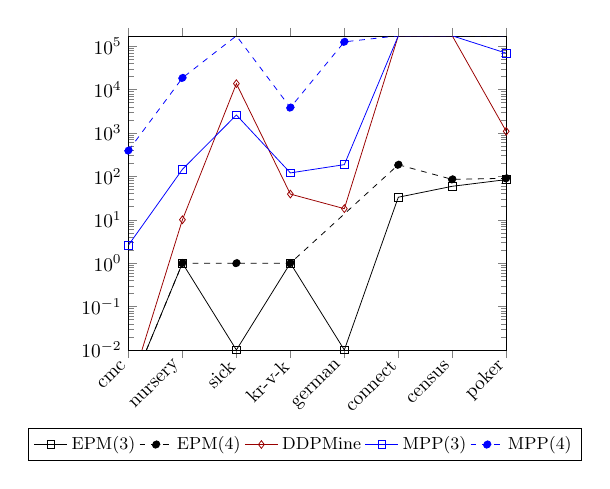
\begin{tikzpicture}[scale = .7]   %
\begin{axis}[
ymin = 0.01, ymax= 170000, legend entries = {EPM(3)\\EPM(4)\\ DDPMine\\ MPP(3)\\MPP(4)\\},ymode=log, %ylabel = Mining Time (Seconds),
legend columns=5, 
legend style={at={(1.2,-0.25)},font=\small}, legend cell align=center,
 draw=none,
 xtick=data,
 xticklabel = {\benchmark{\tick}},
 xtick align=outside,
 ytick align=inside,
 x tick label style={rotate=45,anchor=east},
 title style={font=\Large},
 ylabel near ticks,
 enlarge x limits=false,
xtick distance={400},
 symbolic x coords={cmc,nursery,sick,kr-v-k,german,connect,census,poker},
 ymajorgrids=true,
 grid = none,
 ]
\addplot[
    solid,
    color=black,
    mark=square,
    ]
    coordinates {
    (cmc, 0.001)(nursery, 1)(sick, 0.01)(kr-v-k, 1)(german, 0.01)(connect, 33)(census, 59)(poker, 84)
    };
    \addplot[
    dashed,
    color=black,
    mark=*,
    ]
    coordinates {
    (cmc, 0.001)(nursery, 1)(sick, 1)(kr-v-k, 1)(german,0)(connect, 185)(census, 85)(poker, 90)};
   %     \addplot[
   % dashed,
   % color=black,
   % mark=triangle,
   % ]
   % coordinates {
   % (cmc, 0.001)(nursery, 1)(sick, 3)(kr-v-k, 2)(german,3)(connect, 108)(census, 269)(poker, 238)};
    \addplot[
    solid,
    color=red!60!black,
    mark=diamond,
    ]
    coordinates {
    (cmc, 0.001)(nursery, 10)(sick, 13663)(kr-v-k, 39)(german, 18)(connect, 172800)(census, 172800)(poker, 1090) };
    \addplot[
    color=blue,
    mark=square,
    ]
    coordinates {
    (cmc, 2.6)(nursery, 145)(sick, 2589)(kr-v-k, 120)(german, 186)(connect, 172800)(census, 172800)(poker,68794) };
    \addplot[
    dashed,
    color=blue,
    mark=*,
    ]
    coordinates {
    (cmc, 394)(nursery, 18515)(sick, 172800)(kr-v-k, 3833)(german,125514)(connect, 172800)(census, 172800)(poker, 172800) };

 \end{axis}
\end{tikzpicture}
\end{center}
%}
\caption{Comparison of mining times (seconds).}
\label{fig:all}
\end{figure}
Figure~\ref{fig:all} compares EPM mining time (in seconds) with those of DDPMine and MPP.
The parameter in the parentheses is the pattern size threshold, e.g.\ $\Theta_l=4$ for EPM(4).
The experiments that take more than two days are terminated and are not included.
%TODO As can be seen, increasing $\Theta_l$ does not notably affect the running time of EPM 
%on the datasets with smaller search spaces.
%TODO However, on the datasets with a larger number of frequent items, 
%decreasing $\lambda_1$ affects the processing time more than increasing $\Theta_l$. 
EPM is notably faster in comparison to the other two approaches.
It is notable that the examined datasets are considerably smaller than the coreference data, which includes more than 33 million samples and 200 frequent feature-values.
\begin{tabular}{|p{0.14\textwidth}|p{0.14\textwidth}|p{0.06\textwidth}|p{0.06\textwidth}|p{0.07\textwidth}|p{0.08\textwidth}|}
\hline
%\multicolumn{1}{|c|}{Corpus} &  \multicolumn{1}{c|}{Texts count} &  \multicolumn{1}{c|}{Mentions count} &  \multicolumn{1}{c|}{Chains count} 
Training corpus &  Testing corpus &  avg F1 &  $B^3$ F1 & MUC F1 & CEAFe F1
\\ \hline
AnCor-2019 & RDR & 58.7 & 56.4 & 61.3 & 58.3 \\ \hline
AnCor-2019 & AnCor-2019 & 58.9 & 55.6 & 65.1 & 55.9 \\ \hline
Our corpus  & Our corpus  & 71.0 & 69.6 & 74.2 & 69.3 \\ \hline
Our corpus  & AnCor-2019 & 28.7 & 26.5 & 33.3 & 26.4 \\ \hline
AnCor-2019 + Our corpus  & Our corpus  & 49.4 & 47.6 & 52.2 & 48.4 \\ \hline
AnCor-2019 + Our corpus & AnCor-2019 & 31.8 & 31.4 & 40.7 & 23.3 \\ \hline
\end{tabular}
%
\begin{table}[htbp]
    \begin{center}\footnotesize
    \begin{tabular}{@{}l@{\hskip3pt}|@{\hskip3pt}l@{\hskip3pt}|@{\hskip3pt}r@{\hskip3pt}|@{\hskip3pt}r@{\hskip3pt}||@{\hskip3pt}r@{\hskip3pt}|@{\hskip3pt}r@{}}
         \multicolumn{2}{c}{} & \multicolumn{2}{c}{in-domain} & \multicolumn{2}{c}{out-of-domain} \\ \hline
     %\multicolumn{2}{c|}{} & \multicolumn{1}{c}{CoNLL} & \multicolumn{1}{c||}{LEA} & \multicolumn{1}{c}{CoNLL} & \multicolumn{1}{c}{LEA}  \\ \hline
	 \multicolumn{2}{c}{} & CoNLL & LEA & CoNLL & LEA \\ \hline
          \multicolumn{2}{c}{} & \multicolumn{4}{c}{{pt (Bible)} } \\ \hline
     %top-pairs & $74.48$ & $65.61$ & $74.58$ & $69.81$ & $66.04$ & $51.03$ & $67.73$ & $58.20$\\
	 \multirow{2}{*}{{ deep-coref}}
     &ranking & $75.61$ & $71.00$ & $66.06$ & $57.58$  \\ 
     & +EPM & $76.08$ & $71.13$ & $\boldsymbol{68.14}$ & $\boldsymbol{60.74}$ \\ \hline
     \multirow{2}{*}{{ e2e-coref}} 
     & single& ${77.80}$ & ${73.73}$ & $65.22$ & $58.26$\\ 
	 & ensemble & $\boldsymbol{78.88}$ & $\boldsymbol{74.88}$ & $65.45$ & $59.71$\\
	 \hline 
     \hline
     \multicolumn{2}{c}{} & \multicolumn{4}{c}{{wb (weblog)} } \\ \hline
     %top-pairs & $61.51$ & $48.22$ & $61.58$ & $54.09$ & $58.66$ & $49.65$ & $51.05$ & $50.34$\\
	 \multirow{2}{*}{{ deep-coref}}
     &ranking & $61.46$ & $53.75$ & $57.17$ & $48.74$ \\ 
     &+EPM & $61.97$ & ${53.93}$ & $\boldsymbol{61.52}$ & $\boldsymbol{53.78}$ \\ \hline
     \multirow{2}{*}{{ e2e-coref}}
     &single & ${62.02}$ & $53.09$ & $60.69$ & $52.69$\\ 
	 &ensemble & $\boldsymbol{64.76}$ & $\boldsymbol{57.54}$ & $60.99$ & $52.99$\\
	 
     \hline
    \end{tabular}
    \end{center}
    \caption{In-domain and out-of-domain evaluations for the pt and wb genres of the CoNLL test set.
    The highest scores are boldfaced.
    }
    \label{tab:cross_genre_enhanced_1}
\end{table}
\subsection{Impact on Generalization}
\label{ch:improvements:generalization}
We use the same setup as that of \newcite{moosavi17b} for evaluating generalization 
including (1) training on the CoNLL data and testing on WikiCoref\footnote{WikiCoref only contains 30 documents, which is not enough for training neural coreference resolvers.}
and (2) excluding a genre of the CoNLL data from training and development sets 
and testing on the excluded genre. Similar to \newcite{moosavi17b}, we use the \emph{pt} and \emph{wb} genres for the latter evaluation setup.  
%Following \newcite{moosavi17b}, we use WikiCoref because it has compatible annotation guidelines with CoNLL. 

The results of the first evaluation setup are shown in Table~\ref{tab:out-domain-deep-coref}.
The best performance on WikiCoref is achieved by \newcite{ghaddar16a} (``G\&L'' in Table~\ref{tab:out-domain-deep-coref})
who introduced WikiCoref and design a domain-specific coreference resolver that makes use of 
the Wikipedia markups of a document as well as links to Freebase, which are annotated in WikiCoref.

Incorporating EPM feature-values improves the performance by about three points.
While ``+EPM'' does not use the WikiCoref data during training, and unlike ``G\&L'', it does not employ any domain-specific features,
it achieves on-par performance with that of ``G\&L''.
%We also observe that ``+EPM'' performance is about two point better than ``+linguistic'' (Table~\ref{tab:out_of_domain_linguistics}) on WikiCoref.
This indeed shows the effectiveness of informative feature-values in improving generalization.

%In order to show that the improved generalization is due to incorporating 
%informative feature-values, and not any additional linguistic feature, we also report the performance of ``+all'', 
%i.e.\ ``top-pairs'' in which the feature set of Section~\ref{sect:base_features} is employed.
%As we see, ``+all'' performance is slightly better than ``top-pairs''.
%However, the improvements are not as substantial as those of ``+EPM''. 

%The results of e2e-coref ``single'' vs.\ ``ensemble'' show the effectiveness of ensemble methods for improving generalization.
%By combining ensemble methods, e.g.\ \cite{leekenton17,uryupina-moschitti:2017:CoNLL}, 
%and informative feature-values we can further improve the generalization.
%using an ensemble of ``+EPM'' models is a possible way to further improve the results.

The second set of generalization experiments is reported in Table~\ref{tab:cross_genre_enhanced_1}. 
``in-domain'' columns show the results when the evaluation genres were included in training and development sets 
while the ``out-of-domain'' columns show the results when the evaluation genres were excluded.
As we can see, ``+EPM'' generalizes best, and in out-of-domain evaluations, it considerably outperforms the ensemble model of e2e-coref, which has the best performance on the CoNLL test set. 
%\section{Summary and discussion}\label{s:disc}

In this work we introduced an attack that allows an adversary to violate the 
  guarantees of MPM systems by leveraging users' friends.
We also proposed several mitigations, but our proposals satisfy only two out 
  of three desirable properties: privacy (leak no information), low 
  communication overhead (i.e., clients need not send many messages per round), 
  and low latency (friends get to talk to each other often).
The most pragmatic of our solutions requires bounding the maximum number of 
  friends that a client can have.

Even with our mitigations, compromised friends are a liability and can be
  used to learn sensitive information through other means.
For example, if a user is uncharacteristically slow to respond to a 
  compromised friend's message (a user's response pattern could be constructed over
  many prior interactions), this anomaly in itself leaks information.
We believe that understanding the impact of this type of attack in
  practice is a promising avenue for future work.

\section{CONCLUSION}
\label{sec:conclusion}

% \Ram{Want to mention that we can do parameteric uncertainty \cite{mohan2016convex}, hybrid \cite{shia2014convex}, and alpha confidence \cite{holmes2016convex}
% Also we can pose the optimization problem using convex optimization based methods \cite{zhao2016control,zhao2017optimal}.}

This paper presents a method to plan safe trajectories with obstacle avoidance for autonomous vehicles.
This approach is able to guarantee safety in arbitrary environments for multiple, static obstacles.
The method begins with computing the forward reachable set (FRS) of parameterized trajectories that a vehicle can realize.
This set is computed in continuous space and time, and is robust to model uncertainty between the dynamics of the vehicle's mid- and low-level controllers.

As an example, we use a kinematic Dubin's car and dynamic unicycle model as low- and high-fidelity models.
At runtime, the FRS is intersected with obstacles to eliminate unsafe trajectories, and an optimal trajectory is chosen from the remaining, safe trajectories.
This method is proven to ensure vehicle safety for present and future static obstacles by considering the time required for path planning, the time required to stop the vehicle, and the error between the low- and high-fidelity models.
One thousand simulations with randomly-located obstacles were run to show the effectiveness of this method. 

%We are preparing a Segway as a platform to demonstrate this method on a real system.
%We will also apply this method to higher degree-of-freedom vehicle models in both simulation and experiments to further develop robustness to environmental and dynamic uncertainty.

The next step in applying this method is to expand the error function $g$ beyond modeling uncertainty.
To reduce the conservativeness of the approach, we plan to explore extension to the FRS computation that incorporate confidence level sets \cite{mohan2016convex,holmes2016convex}.
The error function $g$ can also be improved by considering time variation of trajectory parameters across planning steps by posing the FRS computation as a hybrid problem \cite{shia2014convex}.
Finally, we plan to use convex optimization to find a global solution to the nonlinear trajectory optimization problem at each planning step \cite{zhao2016control,zhao2017optimal}.

\section*{Acknowledgments} The authors would like to thank Mark-Christoph M\"uller, Benjamin Heinzerling, Alex Judea, Steffen Eger and the anonymous reviewers for their helpful comments and feedbacks. 
This work has been supported by the Klaus Tschira Foundation, Heidelberg,
Germany and the German Research
Foundation (DFG) as part of the Research Training Group
“Adaptive  Preparation  of  Information  from  Heterogeneous  Sources”  (AIPHES) under  grant  No.
GRK 1994/1. 

\bibliographystyle{acl_natbib_nourl}
\bibliography{mybib}



\end{document}
